\section{\ac{SAT}-solvers}

SMT vs. SAT is like high level \ac{PL} vs. assembly language.
The latter can be much more efficient, but it's hard to program in it.

SAT is abbreviation of ``Boolean satisfiability problem''.
The problem is to find such a set of variables, which, if plugged into boolean expression, will result in ``true''.

\subsection{CNF form}

\ac{CNF}\footnote{\url{https://en.wikipedia.org/wiki/Conjunctive_normal_form}} is a \textit{normal form}.

% TODO recheck
% TODO write abt it!
%\textit{normal form} is somewhat similar to polynomials in algebra. 
%What is polynomial?
%It is a standard way to express unsystematic equations like $2x \cdot x$ as $3x$ polynomial, 
%and so you will be able to apply some operations to polynomials like summing, etc.

Any boolean expression can be converted to \textit{normal form} and \ac{CNF} is one of them.
The \ac{CNF} expression is a bunch of clauses (sub-expressions) constisting of terms (variables), ORs and NOTs, 
all of which are then glueled together with AND into a full expression.
There is a way to memorize it: \ac{CNF} is ``AND of ORs'' (or ``product of sums'') and \ac{DNF} is ``OR of ANDs'' (or ``sum of products'').

Example is: $(\neg A \vee B) \wedge (C \vee \neg D)$.

$\vee$ stands for OR (logical disjunction\footnote{\url{https://en.wikipedia.org/wiki/Logical_disjunction}}), 
``+'' sign is also sometimes used for OR.

$\wedge$ stands for AND (logical conjunction\footnote{\url{https://en.wikipedia.org/wiki/Logical_conjunction}}).
It is easy to memorize: $\wedge$ looks like ``A'' letter.
``$\cdot$'' is also sometimes used for AND.

$\neg$ is negation (NOT).

% TODO A/B is the first clause, C/D is second

\subsection{Example: 2-bit adder}
\label{adder}

\ac{SAT}-solver is merely a solver of huge boolean equations in CNF form.
It just gives the answer, if there is a set of input values which can satisfy CNF expression, and what input values must be.

Here is a 2-bit adder for example:

\begin{figure}[ht!]
\centering
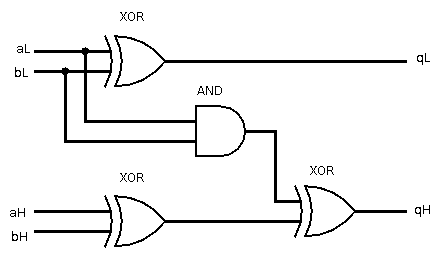
\includegraphics[scale=0.75]{SAT/adder_logisim.png}
\caption{2-bit adder circuit}
\end{figure}

The adder in its simplest form: it has no carry-in and carry-out, and it has 3 XOR gates and one AND gate.
Let's try to figure out, which sets of input values will force adder to set both two output bits?
By doing quick memory calculation, we can see that there are 4 ways to do so: $0+3=3$, $1+2=3$, $2+1=3$, $3+0=3$.
Here is also truth table, with these rows highlighted:

\newcommand{\HLcell}{\cellcolor{blue!25}}

\begin{center}
\begin{doublespace}
\noindent\(\begin{array}{l|llllll}
  & \text{aH} & \text{aL} & \text{bH} & \text{bL} & \text{qH} & \text{qL} \\
\hline
 \text{3+3 = 6 $\equiv $ 2 (mod 4)} & 1 & 1 & 1 & 1 & 1 & 0 \\
 \text{3+2 = 5 $\equiv $ 1 (mod 4)} & 1 & 1 & 1 & 0 & 0 & 1 \\
 \text{3+1 = 4 $\equiv $ 0 (mod 4)} & 1 & 1 & 0 & 1 & 0 & 0 \\
 \text{\HLcell{}3+0 = 3 $\equiv $ 3 (mod 4)} & \HLcell{}1 & \HLcell{}1 & \HLcell{}0 & \HLcell{}0 & \HLcell{}1 & \HLcell{}1 \\
 \text{2+3 = 5 $\equiv $ 1 (mod 4)} & 1 & 0 & 1 & 1 & 0 & 1 \\
 \text{2+2 = 4 $\equiv $ 0 (mod 4)} & 1 & 0 & 1 & 0 & 0 & 0 \\
 \text{\HLcell{}2+1 = 3 $\equiv $ 3 (mod 4)} & \HLcell{}1 & \HLcell{}0 & \HLcell{}0 & \HLcell{}1 & \HLcell{}1 & \HLcell{}1 \\
 \text{2+0 = 2 $\equiv $ 2 (mod 4)} & 1 & 0 & 0 & 0 & 1 & 0 \\
 \text{1+3 = 4 $\equiv $ 0 (mod 4)} & 0 & 1 & 1 & 1 & 0 & 0 \\
 \text{\HLcell{}1+2 = 3 $\equiv $ 3 (mod 4)} & \HLcell{}0 & \HLcell{}1 & \HLcell{}1 & \HLcell{}0 & \HLcell{}1 & \HLcell{}1 \\
 \text{1+1 = 2 $\equiv $ 2 (mod 4)} & 0 & 1 & 0 & 1 & 1 & 0 \\
 \text{1+0 = 1 $\equiv $ 1 (mod 4)} & 0 & 1 & 0 & 0 & 0 & 1 \\
 \text{\HLcell{}0+3 = 3 $\equiv $ 3 (mod 4)} & \HLcell{}0 & \HLcell{}0 & \HLcell{}1 & \HLcell{}1 & \HLcell{}1 & \HLcell{}1 \\
 \text{0+2 = 2 $\equiv $ 2 (mod 4)} & 0 & 0 & 1 & 0 & 1 & 0 \\
 \text{0+1 = 1 $\equiv $ 1 (mod 4)} & 0 & 0 & 0 & 1 & 0 & 1 \\
 \text{0+0 = 0 $\equiv $ 0 (mod 4)} & 0 & 0 & 0 & 0 & 0 & 0 \\
\end{array}\)
\end{doublespace}
\end{center}


Let's find, what \ac{SAT}-solver can say about it?

First, we should represent our 2-bit adder as \ac{CNF} expression.

Using Wolfram Mathematica, we can express 1-bit expression for both adder outputs:\\
\\
\textbf{\texttt{In[]:=AdderQ0[aL$\_$,bL$\_$]=Xor[aL,bL]}} \\
\textbf{\texttt{Out[]:=aL $\veebar$ bL}} \\
\\
\textbf{\texttt{In[]:=AdderQ1[aL$\_$,aH$\_$,bL$\_$,bH$\_$]=Xor[And[aL,bL],Xor[aH,bH]]}} \\
\textbf{\texttt{Out[]:=aH $\veebar$ bH $\veebar$ (aL \&\& bL)}} \\
\\
We need such expression, where both parts will generate 1's.
Let's use Wolfram Mathematica find all instances of such expression (I glueled both parts with And): \\
\\
\textbf{\texttt{In[]:=Boole[SatisfiabilityInstances[And[AdderQ0[aL,bL],AdderQ1[aL,aH,bL,bH]],\{aL,aH,bL,bH\},4]]}} \\
\textbf{\texttt{Out[]:=\{1,1,0,0\},\{1,0,0,1\},\{0,1,1,0\},\{0,0,1,1\}}} \\
\\
Yes, indeed, Mathematica says, there are 4 inputs which will lead to the result we need.
So, Mathematica can also be used as \ac{SAT} solver.

Nevertheless, let's proceed to \ac{CNF} form. Using Mathematica again, let's convert our expression to \ac{CNF} form:\\
\\
\textbf{\texttt{In[]:=cnf=BooleanConvert[And[AdderQ0[aL,bL],AdderQ1[aL,aH,bL,bH]],``CNF'']}} \\
\textbf{\texttt{Out[]:=(!aH $\|$ !bH) \&\& (aH $\|$ bH) \&\& (!aL $\|$ !bL) \&\& (aL $\|$ bL)}} \\
\\
Looks more complex. The reason of such verbosity is that \ac{CNF} form doesn't allow XOR operations.
% FIXME: TeX form of the expression!

\subsubsection{MiniSat}

For starters, we can try MiniSat\footnote{\url{http://minisat.se/MiniSat.html}}.
The standard way to encode \ac{CNF} expression for MiniSat is to enumerate all OR parts at each line.
Also, MiniSat doesn't support variable names, just numbers.
Let's enumerate our variables: 1 will be aH, 2 -- aL, 3 -- bH, 4 -- bL.

Here is what I've got when I converted Mathematica expression to the MiniSat input file:

\lstinputlisting{SAT/adder.cnf}

Two 4's at the first lines are number of variables and number of clauses respectively.
There are 4 lines then, each for each OR clause.
Minus before variable number meaning that the variable is negated.
Absence of minus -- not negated.
Zero at the end is just terminating zero, meaning end of the clause.

In other words, each line is OR-clause with optional negations,
and the task of MiniSat is to find such set of input, which can satisfy all lines in the input file.

That file I named as \textit{adder.cnf} and now let's try MiniSat:

\begin{lstlisting}
% minisat -verb=0 adder.cnf results.txt
SATISFIABLE
\end{lstlisting}

The results are in \textit{results.txt} file:

\begin{lstlisting}
SAT
-1 -2 3 4 0
\end{lstlisting}

This means, if the first two variables (aH and aL) will be \textit{false}, and the last two variables (bH and bL) will be set to \textit{true},
the whole \ac{CNF} expression is satisfiable.
Seems to be true: if bH and bL are the only inputs set to \textit{true}, both resulting bits are also has \textit{true} states.

Now how to get other instances? \ac{SAT}-solvers, like \ac{SMT} solvers, produce only one solution (or \textit{instance}).

MiniSat uses \ac{PRNG} and its initial seed can be set explicitely. I tried different values, but result is still the same.
Nevertheless, CryptoMiniSat in this case was able to show all possible 4 instances, in chaotic order, though.
So this is not very robust way.

Perhaps, the only known way is to negate solution clause and add it to the input expression.
We've got \TT{-1 -2 3 4}, 
now we can negate all values in it (just toggle minuses: \TT{1 2 -3 -4}) and add it to the end of the input file:

\begin{lstlisting}
p cnf 4 5
-1 -3 0
1 3 0
-2 -4 0
2 4 0
1 2 -3 -4
\end{lstlisting}

Now we've got another result:

\begin{lstlisting}
SAT
1 2 -3 -4 0
\end{lstlisting}

This means, aH and aL must be both \textit{true} and bH and bL must be \textit{false}, to satisfy the input expression.
Let's negate this clause and add it again:

\begin{lstlisting}
p cnf 4 6
-1 -3 0
1 3 0
-2 -4 0
2 4 0
1 2 -3 -4
-1 -2 3 4 0
\end{lstlisting}

The result is:

\begin{lstlisting}
SAT
-1 2 3 -4 0
\end{lstlisting}

aH=false, aL=true, bH=true, bL=false. This is also correct, according to our truth table.

Let's add it again:

\begin{lstlisting}
p cnf 4 7
-1 -3 0
1 3 0
-2 -4 0
2 4 0
1 2 -3 -4
-1 -2 3 4 0
1 -2 -3 4 0
\end{lstlisting}

\begin{lstlisting}
SAT
1 -2 -3 4 0
\end{lstlisting}

\textit{aH=true, aL=false, bH=false, bL=true.} This is also correct.

This is fourth result. There are shouldn't be more. What if to add it?

\begin{lstlisting}
p cnf 4 8
-1 -3 0
1 3 0
-2 -4 0
2 4 0
1 2 -3 -4
-1 -2 3 4 0
1 -2 -3 4 0
-1 2 3 -4 0
\end{lstlisting}

Now MiniSat just says ``UNSATISFIABLE'' without any additional information in the resulting file.

Our example is tiny, but MiniSat can work with huge \ac{CNF} expressions.

\subsubsection{CryptoMiniSat}

XOR operation is absent in \ac{CNF} form, but crucial in cryptographical algorithms.
Simplest possible way to represent single XOR operation in \ac{CNF} form is:
$(\neg x \vee \neg y) \wedge (x \vee y)$ -- not that small expression, 
though, many XOR operations in single expression can be optimized better.

One significant difference between MiniSat and CryptoMiniSat is that
the latter supports clauses with XOR operations instead of ORs,
because CryptoMiniSat has aim to analyze crypto algorithms\footnote{\url{http://www.msoos.org/xor-clauses/}}.
XOR clauses are handled by CryptoMiniSat in a special way without translating to OR clauses.

You need just to prepend a clause with ``x'' in \ac{CNF} file and OR clause is then treated as XOR clause by CryptoMiniSat.
As of 2-bit adder, this smallest possible XOR-CNF expression can be used to find all inputs where both output adder bits are set:

$(aH \oplus bH) \wedge (aL \oplus bL)$

This is \TT{.cnf} file for CryptoMiniSat:

\begin{lstlisting}
p cnf 4 2
x1 3 0
x2 4 0
\end{lstlisting}

Now I run CryptoMiniSat with various random values to initialize its \ac{PRNG} \dots

\begin{lstlisting}
% cryptominisat4 --verb 0 --random 0 XOR_adder.cnf
s SATISFIABLE
v 1 2 -3 -4 0
% cryptominisat4 --verb 0 --random 1 XOR_adder.cnf
s SATISFIABLE
v -1 -2 3 4 0
% cryptominisat4 --verb 0 --random 2 XOR_adder.cnf
s SATISFIABLE
v 1 -2 -3 4 0
% cryptominisat4 --verb 0 --random 3 XOR_adder.cnf
s SATISFIABLE
v 1 2 -3 -4 0
% cryptominisat4 --verb 0 --random 4 XOR_adder.cnf
s SATISFIABLE
v -1 2 3 -4 0
% cryptominisat4 --verb 0 --random 5 XOR_adder.cnf
s SATISFIABLE
v -1 2 3 -4 0
% cryptominisat4 --verb 0 --random 6 XOR_adder.cnf
s SATISFIABLE
v -1 -2 3 4 0
% cryptominisat4 --verb 0 --random 7 XOR_adder.cnf
s SATISFIABLE
v 1 -2 -3 4 0
% cryptominisat4 --verb 0 --random 8 XOR_adder.cnf
s SATISFIABLE
v 1 2 -3 -4 0
% cryptominisat4 --verb 0 --random 9 XOR_adder.cnf
s SATISFIABLE
v 1 2 -3 -4 0
\end{lstlisting}

Nevertheless, all 4 possible solutions are:

\begin{lstlisting}
v -1 -2 3 4 0
v -1 2 3 -4 0
v 1 -2 -3 4 0
v 1 2 -3 -4 0
\end{lstlisting}

\dots the same as reported by MiniSat.

\subsection{Picosat}

At least Picosat can enumerate all possible solutions without crutches I just shown:

\begin{lstlisting}
% picosat --all adder.cnf
s SATISFIABLE
v -1 -2 3 4 0
s SATISFIABLE
v -1 2 3 -4 0
s SATISFIABLE
v 1 2 -3 -4 0
s SATISFIABLE
v 1 -2 -3 4 0
s SOLUTIONS 4
\end{lstlisting}

% subsections:
\subsection{Eight queens puzzle}
\label{EightQueens}

Eight queens is a very popular puzzle and often used for measuring performance of SAT solvers.
The problem is to place 8 queens on chess board so they will not attack each other.
For example:

\begin{lstlisting}
| | | |*| | | | |
| | | | | | |*| |
| | | | |*| | | |
| |*| | | | | | |
| | | | | |*| | |
|*| | | | | | | |
| | |*| | | | | |
| | | | | | | |*|
\end{lstlisting}

Let's try to figure out how to solve it.

\subsubsection{POPCNT1}
\label{POPCNTOne}

One important function we will (often) use is \TT{POPCNT1}.
This is a function which returns \textit{True} if one single of inputs is \textit{True} and others are \textit{False}.
It will return \textit{False} otherwise.

In my other examples, I've used Wolfram Mathematica to generate CNF clauses for it, for example: \ref{minesweeper_SAT}.
What expression Mathematica offers as \TT{POPCNT1} function with 8 inputs?

\begin{lstlisting}
(!a||!b)&&(!a||!c)&&(!a||!d)&&(!a||!e)&&(!a||!f)&&(!a||!g)&&(!a||!h)&&(a||b||c||d||e||f||g||h)&&
(!b||!c)&&(!b||!d)&&(!b||!e)&&(!b||!f)&&(!b||!g)&&(!b||!h)&&(!c||!d)&&(!c||!e)&&(!c||!f)&&(!c||!g)&&
(!c||!h)&&(!d||!e)&&(!d||!f)&&(!d||!g)&&(!d||!h)&&(!e||!f)&&(!e||!g)&&(!e||!h)&&(!f||!g)&&(!f||!h)&&(!g||!h)
\end{lstlisting}

We can clearly see that the expression constisting of all possible variable pairs (negated) plus
enumeration of all variables (non-negated).
In plain English terms, this means: ``no pair can be equal to two \textit{True}'s \textit{AND} at least one \textit{True}
must be present among all variables''.

This is how it works: if two variables will be \textit{True}, negated they will be both \textit{False},
and this clause will not be evaluated
to \textit{True}, which is our ultimate goal.
If one of variables is \textit{True}, both negated will produce one \textit{True} and one \textit{False} (fine).
If both variables are False, both negated will produce two \textit{True's} (again, fine).

Here is how I can generate clauses for the function using \textit{itertools} module from Python,
which provides many important functions from combinatorics:

\begin{lstlisting}
    # naive/pairwise encoding   
    def AtMost1(self, lst):
        for pair in itertools.combinations(lst, r=2):
            self.add_clause([self.neg(pair[0]), self.neg(pair[1])])
        
    def POPCNT1(self, lst):
        self.AtMost1(lst)
        self.OR_always(lst)
\end{lstlisting}

\TT{AtMost1()} function enumerates all possible pairs using \textit{itertools} function
\textit{combinations()}.

\TT{POPCNT1()} function does the same, but also adds a final clause, which forces at least one
\textit{True} variable to be present.

What clauses will be generated for 5 variables (1..5)?

\lstinputlisting{SAT/8queens/popcnt1.cnf}

Yes, these are all possible pairs of 1..5 numbers + all 5 numbers.

We can get all solutions using Picosat:

\begin{lstlisting}
% picosat --all popcnt1.cnf
s SATISFIABLE
v -1 -2 -3 -4 5 0
s SATISFIABLE
v -1 -2 -3 4 -5 0
s SATISFIABLE
v -1 -2 3 -4 -5 0
s SATISFIABLE
v -1 2 -3 -4 -5 0
s SATISFIABLE
v 1 -2 -3 -4 -5 0
s SOLUTIONS 5
\end{lstlisting}

5 possible solutions indeed.

\subsubsection{Eight queens}

Now let's get back to eight queens.

We can assign 64 variables to $8 \cdot 8=64$ cells.
Cell occuppied with queen will be \textit{True}, vacant cell will be \textit{False}.

The problem of placing non-attacking (each other) queens on chess board (of any size) can be stated in plain English like this:
\begin{itemize}
\item one single queen must be present at each row;

\item one single queen must be present at each column;

\item zero or one queen must be present at each diagonal (empty diagonals can be present in valid solution).
\end{itemize}

These rules can be translated like that:

\begin{itemize}
\item POPCNT1(each row)==\textit{True}

\item POPCNT1(each column)==\textit{True}

\item AtMost1(each diagonal)==\textit{True}
\end{itemize}

Now all we need is to enumerate rows, columns and diagonals and gather all clauses:

\lstinputlisting{SAT/8queens/8queens.py}
( \url{https://github.com/DennisYurichev/SAT_SMT_article/blob/master/SAT/8queens/8queens.py} )

Perhaps, \TT{gen\_diagonal()} function is not very aesthetically appealing: it enumerates also subdiagonals
of already enumerated longer diagonals.
To prevent presence of duplicate clauses, \textit{clauses} global variable is not a list, rather set, which allows
only unique data to be present there.

Also, I've used \TT{AtMost1} for each column, this will help to produce slightly lower number of clauses.
Each column will have a queen anyway, this is implied from the first rule (\TT{POPCNT1} for each row).

After running, we got CNF file with 64 variables and 736 clauses (\url{https://github.com/DennisYurichev/SAT_SMT_article/blob/master/SAT/8queens/8queens.cnf}).
Here is one solution:

\begin{lstlisting}
% python 8queens.py
len(clauses)= 736
| | | |*| | | | |
| | | | | | |*| |
| | | | |*| | | |
| |*| | | | | | |
| | | | | |*| | |
|*| | | | | | | |
| | |*| | | | | |
| | | | | | | |*|
\end{lstlisting}

How many possible solutions are there?
Picosat tells 92, which is indeed correct number of solutions (\url{https://oeis.org/A000170}).

Performance of Picosat is not impressive, probably because it has to output all the solutions.
It took 34 seconds on my ancient Intel Atom 1.66GHz netbook to enumerate all solutions for $11 \cdot 11$ chess board
(2680 solutions),
which is way slower than my straigt brute-force program: \url{https://yurichev.com/blog/8queens/}.
Nevertheless, it's lighting fast (as other SAT solvers) in finding first solution.

The SAT instance is also small enough to be easily solved by my simplest possible backtracking SAT solver:
\ref{SAT_backtrack}.

\subsubsection{Counting all solutions}

We get a solution, negate it and add as a new constraint.
In plain English language this sounds ``find a solution, which is also can't be equal to the recently found/added''.
We add them consequently and the process is slowing---just because a problem (\textit{instance}) is growing and SAT solver
experience hard times in find yet another solution.

\subsubsection{Skipping symmetrical solutions}

We can also add rotated and reflected (horizontally) solution, so to skip symmetrical solutions.
By doing so, we're getting 12 solutions for 8*8 board, 46 for 9*9 board, etc.
This is \url{https://oeis.org/A002562}.


\subsection{Zebra puzzle as a SAT problem}
\label{Zebra_SAT}

Let's try to solve Zebra puzzle (\ref{zebra_SMT}) in SAT.

I would define each variable as vector of 5 variables, as I did before in Sudoku solver: \ref{Sudoku_SAT}.

I also use \TT{POPCNT1} function, but unlike previous example, I used Wolfram Mathematica to generate it in CNF form:

\begin{lstlisting}
In[]:= tbl1=Table[PadLeft[IntegerDigits[i,2],5] ->If[Equal[DigitCount[i,2][[1]],1],1,0],{i,0,63}]
Out[]= {{0,0,0,0,0}->0,
{0,0,0,0,1}->1,
{0,0,0,1,0}->1,
{0,0,0,1,1}->0,
{0,0,1,0,0}->1,
{0,0,1,0,1}->0,

...

{1,1,1,1,0}->0,
{1,1,1,1,1}->0}

In[]:= BooleanConvert[BooleanFunction[tbl1,{a,b,c,d,e}],"CNF"]
Out[]= (!a||!b)&&(!a||!c)&&(!a||!d)&&(!a||!e)&&(a||b||c||d||e)&&(!b||!c)&&(!b||!d)&&(!b||!e)&&(!c||!d)&&(!c||!e)&&(!d||!e)
\end{lstlisting}

Also, as I suggested before (\ref{OR_in_POPCNT1}), I used \textit{OR} operation as the second step.

\begin{lstlisting}
def mathematica_to_CNF (s, d):
    for k in d.keys():
        s=s.replace(k, d[k])
    s=s.replace("!", "-").replace("||", " ").replace("(", "").replace(")", "")
    s=s.split ("&&")
    return s

def add_popcnt1(v1, v2, v3, v4, v5):
    global clauses
    s="(!a||!b)&&" \
      "(!a||!c)&&" \
      "(!a||!d)&&" \
      "(!a||!e)&&" \
      "(!b||!c)&&" \
      "(!b||!d)&&" \
      "(!b||!e)&&" \
      "(!c||!d)&&" \
      "(!c||!e)&&" \
      "(!d||!e)&&" \
      "(a||b||c||d||e)"

    clauses=clauses+mathematica_to_CNF(s, {"a":v1, "b":v2, "c":v3, "d":v4, "e":v5})

...

# k=tuple: ("high-level" variable name, number of bit (0..4))
# v=variable number in CNF
vars={}
vars_last=1

...

def alloc_distinct_variables(names):
    global vars
    global vars_last
    for name in names:
        for i in range(5):
            vars[(name,i)]=str(vars_last)
            vars_last=vars_last+1

        add_popcnt1(vars[(name,0)], vars[(name,1)], vars[(name,2)], vars[(name,3)], vars[(name,4)])

    # make them distinct:
    for i in range(5):
        clauses.append(vars[(names[0],i)] + " " + vars[(names[1],i)] + " " + vars[(names[2],i)] + " " + vars[(names[3],i)] + " " + vars[(names[4],i)])

...

alloc_distinct_variables(["Yellow", "Blue", "Red", "Ivory", "Green"])
alloc_distinct_variables(["Norwegian", "Ukrainian", "Englishman", "Spaniard", "Japanese"])
alloc_distinct_variables(["Water", "Tea", "Milk", "OrangeJuice", "Coffee"])
alloc_distinct_variables(["Kools", "Chesterfield", "OldGold", "LuckyStrike", "Parliament"])
alloc_distinct_variables(["Fox", "Horse", "Snails", "Dog", "Zebra"])

...

\end{lstlisting}

Now we have 5 boolean variables for each \textit{high-level} variable,
and each group of variables will always have distinct values.

Now let's reread puzzle description: ``2.The Englishman lives in the red house.''.
That's easy.
In my Z3 and KLEE examples I just wrote ``Englishman==Red''.
Same story here: we just add a clauses showing that 5 boolean variables for ``Englishman''
must be equal to 5 booleans for ``Red''.

On a lowest CNF level, if we want to say that two variables must be equal to each other, we add two clauses:

$(var1 \vee \neg var2) \wedge (\neg var1 \vee var2)$

That means, both \textit{var1} and \textit{var2} values must be \textit{False} or \textit{True},
but they cannot be different.

\begin{lstlisting}
def add_eq_clauses(var1, var2):
    global clauses
    clauses.append(var1 + " -" + var2)
    clauses.append("-"+var1 + " " + var2)

def add_eq (n1, n2):
    for i in range(5):
        add_eq_clauses(vars[(n1,i)], vars[(n2, i)])

...

# 2.The Englishman lives in the red house.
add_eq("Englishman","Red")

# 3.The Spaniard owns the dog.
add_eq("Spaniard","Dog")

# 4.Coffee is drunk in the green house.
add_eq("Coffee","Green")

...

\end{lstlisting}

Now the next conditions:
``9.Milk is drunk in the middle house.'' (i.e., 3rd house), ``10.The Norwegian lives in the first house.''
We can just assign boolean values directly:

\begin{lstlisting}
# n=1..5
def add_eq_var_n (name, n):
    global clauses
    global vars
    for i in range(5):
        if i==n-1:
            clauses.append(vars[(name,i)]) # always True
        else:
            clauses.append("-"+vars[(name,i)]) # always False

...

# 9.Milk is drunk in the middle house.
add_eq_var_n("Milk",3) # i.e., 3rd house

# 10.The Norwegian lives in the first house.
add_eq_var_n("Norwegian",1)
\end{lstlisting}

For ``Milk'' we will have ``0 0 1 0 0'' value, for ``Norwegian'': ``1 0 0 0 0''.

What to do with this?
``6.The green house is immediately to the right of the ivory house.''
I can construct the following condition:

\begin{lstlisting}
    Ivory      Green
AND(1 0 0 0 0  0 1 0 0 0)
.. OR ..
AND(0 1 0 0 0  0 0 1 0 0)
.. OR ..
AND(0 0 1 0 0  0 0 0 1 0)
.. OR ..
AND(0 0 0 1 0  0 0 0 0 1)
\end{lstlisting}

There is no ``0 0 0 0 1'' for ``Ivory'', because it cannot be the last one.
Now I can convert these conditions to CNF using Wolfram Mathematica:

\begin{lstlisting}
In[]:= BooleanConvert[(a1&& !b1&&!c1&&!d1&&!e1&&!a2&& b2&&!c2&&!d2&&!e2) ||
(!a1&& b1&&!c1&&!d1&&!e1&&!a2&& !b2&&c2&&!d2&&!e2) ||
(!a1&& !b1&&c1&&!d1&&!e1&&!a2&& !b2&&!c2&&d2&&!e2) ||
(!a1&& !b1&&!c1&&d1&&!e1&&!a2&& !b2&&!c2&&!d2&&e2) ,"CNF"]

Out[]= (!a1||!b1)&&(!a1||!c1)&&(!a1||!d1)&&(a1||b1||c1||d1)&&!a2&&(!b1||!b2)&&(!b1||!c1)&&
(!b1||!d1)&&(b1||b2||c1||d1)&&(!b2||!c1)&&(!b2||!c2)&&(!b2||!d1)&&(!b2||!d2)&&(!b2||!e2)&&
(b2||c1||c2||d1)&&(b2||c2||d1||d2)&&(b2||c2||d2||e2)&&(!c1||!c2)&&(!c1||!d1)&&(!c2||!d1)&&
(!c2||!d2)&&(!c2||!e2)&&(!d1||!d2)&&(!d2||!e2)&&!e1
\end{lstlisting}

And here is a piece of my Python code:

\begin{lstlisting}
def add_right (n1, n2):
    global clauses
    s="(!a1||!b1)&&(!a1||!c1)&&(!a1||!d1)&&(a1||b1||c1||d1)&&!a2&&(!b1||!b2)&&(!b1||!c1)&&(!b1||!d1)&&" \
      "(b1||b2||c1||d1)&&(!b2||!c1)&&(!b2||!c2)&&(!b2||!d1)&&(!b2||!d2)&&(!b2||!e2)&&(b2||c1||c2||d1)&&" \
      "(b2||c2||d1||d2)&&(b2||c2||d2||e2)&&(!c1||!c2)&&(!c1||!d1)&&(!c2||!d1)&&(!c2||!d2)&&(!c2||!e2)&&" \
      "(!d1||!d2)&&(!d2||!e2)&&!e1"

    clauses=clauses+mathematica_to_CNF(s, {
	"a1": vars[(n1,0)], "b1": vars[(n1,1)], "c1": vars[(n1,2)], "d1": vars[(n1,3)], "e1": vars[(n1,4)],
	"a2": vars[(n2,0)], "b2": vars[(n2,1)], "c2": vars[(n2,2)], "d2": vars[(n2,3)], "e2": vars[(n2,4)]})

...

# 6.The green house is immediately to the right of the ivory house.
add_right("Ivory", "Green")
\end{lstlisting}

What we will do with that?
``11.The man who smokes Chesterfields lives in the house next to the man with the fox.''
``12.Kools are smoked in the house next to the house where the horse is kept.''

We don't know side, left or right, but we know that they are differ in one.
Here is a clauses I would add:

\begin{lstlisting}
    Chesterfield  Fox
AND(0 0 0 0 1     0 0 0 1 0)
.. OR ..
AND(0 0 0 1 0     0 0 0 0 1)
AND(0 0 0 1 0     0 0 1 0 0)
.. OR ..
AND(0 0 1 0 0     0 1 0 0 0)
AND(0 0 1 0 0     0 0 0 1 0)
.. OR ..
AND(0 1 0 0 0     1 0 0 0 0)
AND(0 1 0 0 0     0 0 1 0 0)
.. OR ..
AND(1 0 0 0 0     0 1 0 0 0)
\end{lstlisting}

I can convert this into CNF using Mathematica again:

\begin{lstlisting}
In[]:= BooleanConvert[(a1&& !b1&&!c1&&!d1&&!e1&&!a2&& b2&&!c2&&!d2&&!e2) ||

(!a1&& b1&&!c1&&!d1&&!e1&&a2&& !b2&&!c2&&!d2&&!e2) ||
(!a1&& b1&&!c1&&!d1&&!e1&&!a2&& !b2&&c2&&!d2&&!e2) ||

(!a1&& !b1&&c1&&!d1&&!e1&&!a2&& b2&&!c2&&!d2&&!e2) ||
(!a1&& !b1&&c1&&!d1&&!e1&&!a2&& !b2&&!c2&&d2&&!e2) ||

(!a1&& !b1&&!c1&&d1&&!e1&&!a2&& !b2&&c2&&!d2&&!e2) ||
(!a1&& !b1&&!c1&&d1&&!e1&&!a2&& !b2&&!c2&&!d2&&e2) ||

(!a1&& !b1&&!c1&&!d1&&e1&&!a2&& !b2&&!c2&&d2&&!e2) ,"CNF"]

Out[]= (!a1||!b1)&&(!a1||!c1)&&(!a1||!d1)&&(!a1||!e1)&&(a1||b1||c1||d1||e1)&&(!a2||b1)&&(!a2||!b2)&&
(!a2||!c2)&&(!a2||!d2)&&(!a2||!e2)&&(a2||b2||c1||c2||d1||e1)&&(a2||b2||c2||d1||d2)&&(a2||b2||c2||d2||e2)&&
(!b1||!b2)&&(!b1||!c1)&&(!b1||!d1)&&(!b1||!e1)&&(b1||b2||c1||d1||e1)&&(!b2||!c2)&&(!b2||!d1)&&(!b2||!d2)&&
(!b2||!e1)&&(!b2||!e2)&&(!c1||!c2)&&(!c1||!d1)&&(!c1||!e1)&&(!c2||!d2)&&(!c2||!e1)&&(!c2||!e2)&&
(!d1||!d2)&&(!d1||!e1)&&(!d2||!e2)
\end{lstlisting}

And here is my code:

\begin{lstlisting}
def add_right_or_left (n1, n2):
    global clauses
    s="(!a1||!b1)&&(!a1||!c1)&&(!a1||!d1)&&(!a1||!e1)&&(a1||b1||c1||d1||e1)&&(!a2||b1)&&" \
      "(!a2||!b2)&&(!a2||!c2)&&(!a2||!d2)&&(!a2||!e2)&&(a2||b2||c1||c2||d1||e1)&&(a2||b2||c2||d1||d2)&&" \
       "(a2||b2||c2||d2||e2)&&(!b1||!b2)&&(!b1||!c1)&&(!b1||!d1)&&(!b1||!e1)&&(b1||b2||c1||d1||e1)&&" \
       "(!b2||!c2)&&(!b2||!d1)&&(!b2||!d2)&&(!b2||!e1)&&(!b2||!e2)&&(!c1||!c2)&&(!c1||!d1)&&(!c1||!e1)&&" \
       "(!c2||!d2)&&(!c2||!e1)&&(!c2||!e2)&&(!d1||!d2)&&(!d1||!e1)&&(!d2||!e2)"
    
    clauses=clauses+mathematica_to_CNF(s, {
	"a1": vars[(n1,0)], "b1": vars[(n1,1)], "c1": vars[(n1,2)], "d1": vars[(n1,3)], "e1": vars[(n1,4)],
	"a2": vars[(n2,0)], "b2": vars[(n2,1)], "c2": vars[(n2,2)], "d2": vars[(n2,3)], "e2": vars[(n2,4)]})

...

# 11.The man who smokes Chesterfields lives in the house next to the man with the fox.
add_right_or_left("Chesterfield","Fox") # left or right

# 12.Kools are smoked in the house next to the house where the horse is kept.
add_right_or_left("Kools","Horse") # left or right
\end{lstlisting}

This is it!
The full source code: \url{https://github.com/DennisYurichev/SAT_SMT_article/blob/master/SAT/zebra/zebra_SAT.py}.

Resulting CNF instance has 125 boolean variables and 511 clauses: \\
\url{https://github.com/DennisYurichev/SAT_SMT_article/blob/master/SAT/zebra/1.cnf}.
It is a piece of cake for any SAT solver.
Even my toy-level SAT-solver (\ref{SAT_backtrack}) can solve it in \textasciitilde{}1 second on my ancient Intel Atom netbook.

And of course, there is only one possible solution, what is acknowledged by Picosat.

\begin{lstlisting}
% python zebra_SAT.py
Yellow 1
Blue 2
Red 3
Ivory 4
Green 5
Norwegian 1
Ukrainian 2
Englishman 3
Spaniard 4
Japanese 5
Water 1
Tea 2
Milk 3
OrangeJuice 4
Coffee 5
Kools 1
Chesterfield 2
OldGold 3
LuckyStrike 4
Parliament 5
Fox 1
Horse 2
Snails 3
Dog 4
Zebra 5
\end{lstlisting}


\subsection{Cracking Minesweeper with SAT solver}
\label{minesweeper_SAT}

See also about cracking it using Z3: \ref{minesweeper_SMT}.

\subsubsection{Simple \textit{population count} function}

First of all, somehow we need to count neighbour bombs.
The counting function is similar to \textit{population count} function.

We can try to make \ac{CNF} expression using Wolfram Mathematica.
This will be a function, returning \textit{True}
if any of 2 bits of 8 inputs bits are \textit{True} and others are \textit{False}.
First, we make truth table of such function:

\begin{lstlisting}
In[]:= tbl2 = 
 Table[PadLeft[IntegerDigits[i, 2], 8] -> 
   If[Equal[DigitCount[i, 2][[1]], 2], 1, 0], {i, 0, 255}]

Out[]= {{0, 0, 0, 0, 0, 0, 0, 0} -> 0, {0, 0, 0, 0, 0, 0, 0, 1} -> 0, 
{0, 0, 0, 0, 0, 0, 1, 0} -> 0, {0, 0, 0, 0, 0, 0, 1, 1} -> 1, 
{0, 0, 0, 0, 0, 1, 0, 0} -> 0, {0, 0, 0, 0, 0, 1, 0, 1} -> 1, 
{0, 0, 0, 0, 0, 1, 1, 0} -> 1, {0, 0, 0, 0, 0, 1, 1, 1} -> 0, 
{0, 0, 0, 0, 1, 0, 0, 0} -> 0, {0, 0, 0, 0, 1, 0, 0, 1} -> 1, 
{0, 0, 0, 0, 1, 0, 1, 0} -> 1, {0, 0, 0, 0, 1, 0, 1, 1} -> 0, 
...
{1, 1, 1, 1, 1, 0, 1, 0} -> 0, {1, 1, 1, 1, 1, 0, 1, 1} -> 0, 
{1, 1, 1, 1, 1, 1, 0, 0} -> 0, {1, 1, 1, 1, 1, 1, 0, 1} -> 0, 
{1, 1, 1, 1, 1, 1, 1, 0} -> 0, {1, 1, 1, 1, 1, 1, 1, 1} -> 0}
\end{lstlisting}

Now we can make \ac{CNF} expression using this truth table:

\begin{lstlisting}
In[]:= BooleanConvert[
 BooleanFunction[tbl2, {a, b, c, d, e, f, g, h}], "CNF"]

Out[]= (! a || ! b || ! c) && (! a || ! b || ! d) && (! a || ! 
    b || ! e) && (! a || ! b || ! f) && (! a || ! b || ! g) && (! 
    a || ! b || ! h) && (! a || ! c || ! d) && (! a || ! c || ! 
    e) && (! a || ! c || ! f) && (! a || ! c || ! g) && (! a || ! 
    c || ! h) && (! a || ! d || ! e) && (! a || ! d || ! f) && (! 
    a || ! d || ! g) && (! a || ! d || ! h) && (! a || ! e || ! 
    f) && (! a || ! e || ! g) && (! a || ! e || ! h) && (! a || ! 
    f || ! g) && (! a || ! f || ! h) && (! a || ! g || ! h) && (a || 
   b || c || d || e || f || g) && (a || b || c || d || e || f || 
   h) && (a || b || c || d || e || g || h) && (a || b || c || d || f ||
    g || h) && (a || b || c || e || f || g || h) && (a || b || d || 
   e || f || g || h) && (a || c || d || e || f || g || 
   h) && (! b || ! c || ! d) && (! b || ! c || ! e) && (! b || ! 
    c || ! f) && (! b || ! c || ! g) && (! b || ! c || ! h) && (! 
    b || ! d || ! e) && (! b || ! d || ! f) && (! b || ! d || ! 
    g) && (! b || ! d || ! h) && (! b || ! e || ! f) && (! b || ! 
    e || ! g) && (! b || ! e || ! h) && (! b || ! f || ! g) && (! 
    b || ! f || ! h) && (! b || ! g || ! h) && (b || c || d || e || 
   f || g || 
   h) && (! c || ! d || ! e) && (! c || ! d || ! f) && (! c || ! 
    d || ! g) && (! c || ! d || ! h) && (! c || ! e || ! f) && (! 
    c || ! e || ! g) && (! c || ! e || ! h) && (! c || ! f || ! 
    g) && (! c || ! f || ! h) && (! c || ! g || ! h) && (! d || ! 
    e || ! f) && (! d || ! e || ! g) && (! d || ! e || ! h) && (! 
    d || ! f || ! g) && (! d || ! f || ! h) && (! d || ! g || ! 
    h) && (! e || ! f || ! g) && (! e || ! f || ! h) && (! e || ! 
    g || ! h) && (! f || ! g || ! h)
\end{lstlisting}

The syntax is similar to C/C++.
Let's check it.

I wrote a Python function to convert Mathematica's output into \ac{CNF} file which can be feeded to SAT solver:

\lstinputlisting{SAT/minesweeper/tst.py}

It replaces a/b/c/... variables to the variable names passed (1/2/3...), reworks syntax, etc.
Here is a result:

\lstinputlisting{SAT/minesweeper/tst1.cnf}

I can run it:

\begin{lstlisting}
% minisat -verb=0 tst1.cnf results.txt
SATISFIABLE

% cat results.txt
SAT
1 -2 -3 -4 -5 -6 -7 8 0
\end{lstlisting}

The variable name in results lacking minus sign is \textit{True}.
Variable name with minus sign is \textit{False}.
We see there are just two variables are \textit{True}: 1 and 8.
This is indeed correct: MiniSat solver found a condition, for which our function returns \textit{True}.
Zero at the end is just a terminal symbol which means nothing.

We can ask MiniSat for another solution, by adding current solution to the input CNF file, but with all variables negated:

\begin{lstlisting}
...
-5 -6 -8 0
-5 -7 -8 0
-6 -7 -8 0
-1 2 3 4 5 6 7 -8 0
\end{lstlisting}

In plain English language, this means ``give me ANY solution which can satisfy all clauses, but also not equal to the last clause we've just added''.

MiniSat, indeed, found another solution, again, with only 2 variables equal to \textit{True}:

\begin{lstlisting}
% minisat -verb=0 tst2.cnf results.txt
SATISFIABLE

% cat results.txt
SAT
1 2 -3 -4 -5 -6 -7 -8 0
\end{lstlisting}

By the way, \textit{population count} function for 8 neighbours (POPCNT8) in CNF form is simplest:

\begin{lstlisting}
a&&b&&c&&d&&e&&f&&g&&h
\end{lstlisting}

Indeed: it's true if all 8 input bits are \textit{True}.

The function for 0 neighbours (POPCNT0) is also simple:

\begin{lstlisting}
!a&&!b&&!c&&!d&&!e&&!f&&!g&&!h
\end{lstlisting}

It means, it will return \textit{True}, if all input variables are \textit{False}.

By the way, POPCNT1 function is also simple:

\begin{lstlisting}
(!a||!b)&&(!a||!c)&&(!a||!d)&&(!a||!e)&&(!a||!f)&&(!a||!g)&&(!a||!h)&&(a||b||c||d||e||f||g||h)&&
(!b||!c)&&(!b||!d)&&(!b||!e)&&(!b||!f)&&(!b||!g)&&(!b||!h)&&(!c||!d)&&(!c||!e)&&(!c||!f)&&(!c||!g)&&
(!c||!h)&&(!d||!e)&&(!d||!f)&&(!d||!g)&&(!d||!h)&&(!e||!f)&&(!e||!g)&&(!e||!h)&&(!f||!g)&&(!f||!h)&&(!g||!h)
\end{lstlisting}

There is just enumeration of all possible pairs of 8 variables (a/b, a/c, a/d, etc), which implies:
no two bits must be present simultaneously in each possible pair.
And there is another clause: ``(a||b||c||d||e||f||g||h)'', which implies:
at least one bit must be present among 8 variables.

And yes, you can ask Mathematica for finding \ac{CNF} expressions for any other truth table.

\subsubsection{Minesweeper}

Now we can use Mathematica to generate all \textit{population count} functions for 0..8 neighbours.

For $9 \cdot 9$ Minesweeper matrix including invisible border, there will be $11 \cdot 11=121$ variables,
mapped to Minesweeper matrix like this:

\begin{lstlisting}
 1    2   3   4   5   6   7   8   9  10  11
12   13  14  15  16  17  18  19  20  21  22
23   24  25  26  27  28  29  30  31  32  33
34   35  36  37  38  39  40  41  42  43  44

...

100 101 102 103 104 105 106 107 108 109 110
111 112 113 114 115 116 117 118 119 120 121
\end{lstlisting}

Then we write a Python script which stacks all \textit{population count} functions:
each function for each known number of neighbours (digit on Minesweeper field).
Each POPCNTx() function takes list of variable numbers and outputs list of clauses to be added to the final \ac{CNF} file.

As of empty cells, we also add them as clauses, but with minus sign, which means, the variable must be \textit{False}.
Whenever we try to place bomb, we add its variable as clause without minus sign, this means the variable must be \textit{True}.

Then we execute external minisat process.
The only thing we need from it is exit code.
If an input \ac{CNF} is \TT{UNSAT}, it returns 20:

We use here the information from the previous solving of Minesweeper: \ref{minesweeper_SMT}.

\lstinputlisting{SAT/minesweeper/minesweeper_SAT.py}

( \url{https://github.com/DennisYurichev/SAT_SMT_article/blob/master/SAT/minesweeper/minesweeper_SAT.py} ) \\
\\
The output \ac{CNF} file can be large, up to $\approx 2000$ clauses, or more, here is an example: \url{https://github.com/DennisYurichev/SAT_SMT_article/blob/master/SAT/minesweeper/sample.cnf}.

Anyway, it works just like my previous Z3Py script:

\begin{lstlisting}
row=1, col=3, unsat!
row=6, col=2, unsat!
row=6, col=3, unsat!
row=7, col=4, unsat!
row=7, col=9, unsat!
row=8, col=9, unsat!
\end{lstlisting}

\dots but it runs way faster, even considering overhead of executing external program.
Perhaps, Z3Py version could be optimized much better?

The files, including Wolfram Mathematica notebook: \url{https://github.com/DennisYurichev/SAT_SMT_article/tree/master/SAT/minesweeper}.


\subsection{Simplest SAT solver in \textasciitilde{}120 lines}
\label{SAT_backtrack}

This is simplest possible backtracking SAT solver written in Python (not a \ac{DPLL} one).
It uses the same backtracking algorithm you can find in many simple Sudoku and 8 queens solvers.
It works significantly slower, but due to its extreme simplicity, it can also count solutions.
For example, it can count all solutions of 8 queens problem (\ref{EightQueens}).

Also, there are 70 solutions for POPCNT4 function
\footnote{\url{https://github.com/DennisYurichev/SAT_SMT_article/blob/master/SAT/backtrack/POPCNT4.cnf}}
(the function is true if any 4 of its input 8 variables are true):

\begin{lstlisting}
SAT
-1 -2 -3 -4 5 6 7 8 0
SAT
-1 -2 -3 4 -5 6 7 8 0
SAT
-1 -2 -3 4 5 -6 7 8 0
SAT
-1 -2 -3 4 5 6 -7 8 0
...

SAT
1 2 3 -4 -5 6 -7 -8 0
SAT
1 2 3 -4 5 -6 -7 -8 0
SAT
1 2 3 4 -5 -6 -7 -8 0
UNSAT
solutions= 70
\end{lstlisting}

It was also tested on my SAT-based Minesweeper cracker (\ref{minesweeper_SAT}),
and finishes in reasonable time (though, slower than MiniSat by a factor of \textasciitilde{}10).

On bigger \ac{CNF} instances, it gets stuck, though.

The source code:

\lstinputlisting{SAT/backtrack/SAT_backtrack.py}

As you can see, all it does is enumerate all possible solutions, but prunes search tree as early as possible.
This is backtracking.

The files: \url{https://github.com/DennisYurichev/SAT_SMT_article/tree/master/SAT/backtrack}.

Some comments: \url{https://www.reddit.com/r/compsci/comments/6jn3th/simplest_sat_solver_in_120_lines/}.


\subsection{Integer factorization using SAT solver}
\label{factor_SAT}

See also: integer factorization using Z3 SMT solver (\ref{factor_Z3}).

We are going to simulate electronic circuit of binary multiplier in SAT and then ask solver, what multiplier's inputs must be so the output will be a desired number?
If this situation is impossible, the desired number is prime.

First we should build multiplier out of adders.

\subsubsection{Binary adder in SAT}

Simple binary adder usually constists of full-adders and one half-adder.
These are basic elements of adders.

% FIXME: TikZ!
\begin{figure}[H]
\centering

\includegraphics[scale=1]{SAT/factor/half_adder.png}
\caption{Half-adder}
\end{figure}

( The image has been taken from \href{https://en.wikipedia.org/wiki/Adder_(electronics)}{Wikipedia}. )

Full-adder:

% FIXME: TikZ!
\begin{figure}[H]
\centering

\includegraphics[scale=1]{SAT/factor/full_adder.png}
\caption{Full-adder}
\end{figure}

( The image has been taken from \href{https://en.wikipedia.org/wiki/Adder_(electronics)}{Wikipedia}. )

Here is a 4-bit ripple-carry adder:

% TikZ!
\begin{lstlisting}
         X3 Y3              X2 Y2              X1 Y1              X0 Y0
         |  |               |  |               |  |               |  |
         v  v               v  v               v  v               v  v
        +----+             +----+             +----+             +----+
Cout <- | FA | <- carry <- | FA | <- carry <- | FA | <- carry <- | HA |
        +----+             +----+             +----+             +----+
          ^                  ^                  ^                  ^
          |                  |                  |                  |
          S3                 S2                 S1                 S0
\end{lstlisting}

It can be used for most tasks.

Here is a 4-bit ripple-carry adder with carry-in:

\begin{lstlisting}
         X3 Y3              X2 Y2              X1 Y1              X0 Y0
         |  |               |  |               |  |               |  |
         v  v               v  v               v  v               v  v
        +----+             +----+             +----+             +----+
Cout <- | FA | <- carry <- | FA | <- carry <- | FA | <- carry <- | FA | <- Cin
        +----+             +----+             +----+             +----+
          ^                  ^                  ^                  ^
          |                  |                  |                  |
          S3                 S2                 S1                 S0
\end{lstlisting}

What carries are?
4-bit adder can sum up two numbers up to 0b1111 (15).
15+15=30 and this is 0b11110, i.e., 5 bits. Lowest 4 bits is a sum.
5th most significant bit is not a part of sum, but is a carry bit.

If you sum two numbers on x86 CPU, CF flag is a carry bit connected to \ac{ALU}.
It is set if a resulting sum is bigger than it can be fit into result.

Now you can also need carry-in.
Again, x86 CPU has ADC instruction, it takes CF flag state.
It can be said, CF flag is connected to adder's carry-in input.
Hence, combining two ADD and ADC instructions you can sum up 128 bits on 64-bit CPU.

By the way, this is a good explanation of "carry-ripple".
The very first full-adder's result is depending on the carry-out of the previous full-adder.
Hence, adders cannot work in parallel.
This is a problem of simplest possible adder, other adders can solve this.

To represent full-adders in CNF form, we can use Wolfram Mathematica.
I've taken truth table for full-adder from \href{https://en.wikipedia.org/wiki/Adder_(electronics)}{Wikipedia}:

% FIXME: table!
\begin{lstlisting}
Inputs 	|  Outputs
--------+----------
A B Cin |  Cout Sum
0 0 0   |  0    0
0 0 1   |  0    1
0 1 0   |  0    1
0 1 1   |  1    0
1 0 0   |  0    1
1 0 1   |  1    0
1 1 0   |  1    0
1 1 1   |  1    1
\end{lstlisting}

In Mathematica, I'm setting "->1" if row is correct and "->0" if not correct.

\begin{lstlisting}
In[59]:= FaTbl = {{0, 0, 0, 0, 0} -> 1, {0, 0, 0, 0, 1} -> 
   0, {0, 0, 0, 1, 0} -> 0, {0, 0, 0, 1, 1} -> 0, {0, 0, 1, 0, 0} -> 
   0, {0, 0, 1, 0, 1} -> 1, {0, 0, 1, 1, 0} -> 0, {0, 0, 1, 1, 1} -> 
   0, {0, 1, 0, 0, 0} -> 0, {0, 1, 0, 0, 1} -> 1, {0, 1, 0, 1, 0} -> 
   0, {0, 1, 0, 1, 1} -> 0, {0, 1, 1, 0, 0} -> 0, {0, 1, 1, 0, 1} -> 
   0, {0, 1, 1, 1, 0} -> 1, {0, 1, 1, 1, 1} -> 0, {1, 0, 0, 0, 0} -> 
   0, {1, 0, 0, 0, 1} -> 1, {1, 0, 0, 1, 0} -> 0, {1, 0, 0, 1, 1} -> 
   0, {1, 0, 1, 0, 0} -> 0, {1, 0, 1, 0, 1} -> 0, {1, 0, 1, 1, 0} -> 
   1, {1, 0, 1, 1, 1} -> 0, {1, 1, 0, 0, 0} -> 0, {1, 1, 0, 0, 1} -> 
   0, {1, 1, 0, 1, 0} -> 1, {1, 1, 0, 1, 1} -> 0, {1, 1, 1, 0, 0} -> 
   0, {1, 1, 1, 0, 1} -> 0, {1, 1, 1, 1, 0} -> 0, {1, 1, 1, 1, 1} -> 1}

...

In[60]:= BooleanConvert[
 BooleanFunction[FaTbl, {a, b, cin, cout, s}], "CNF"]

Out[60]= (! a || ! b || ! cin || s) && (! a || ! b || 
   cout) && (! a || ! cin || cout) && (! a || cout || s) && (a || b ||
    cin || ! s) && (a || b || ! cout) && (a || 
   cin || ! cout) && (a || ! cout || ! s) && (! b || ! cin || 
   cout) && (! b || cout || s) && (b || 
   cin || ! cout) && (b || ! cout || ! s) && (! cin || cout || 
   s) && (cin || ! cout || ! s)
\end{lstlisting}

These clauses can be used as full-adder.

Here is it:

\begin{lstlisting}
    # full-adder, as found by Mathematica using truth table:
    def FA (self, a,b,cin):
        s=self.create_var()
        cout=self.create_var()

        self.add_clause([self.neg(a), self.neg(b), self.neg(cin), s])
        self.add_clause([self.neg(a), self.neg(b), cout])
        self.add_clause([self.neg(a), self.neg(cin), cout])
        self.add_clause([self.neg(a), cout, s])
        self.add_clause([a, b, cin, self.neg(s)])
        self.add_clause([a, b, self.neg(cout)])
        self.add_clause([a, cin, self.neg(cout)])
        self.add_clause([a, self.neg(cout), self.neg(s)])
        self.add_clause([self.neg(b), self.neg(cin), cout])
        self.add_clause([self.neg(b), cout, s])
        self.add_clause([b, cin, self.neg(cout)])
        self.add_clause([b, self.neg(cout), self.neg(s)])
        self.add_clause([self.neg(cin), cout, s])
        self.add_clause([cin, self.neg(cout), self.neg(s)])

        return s, cout
\end{lstlisting}

And the adder:

\begin{lstlisting}
    # bit order: [MSB..LSB]
    # n-bit adder:
    def adder(self, X,Y):
        assert len(X)==len(Y)
        # first full-adder could be half-adder
        # start with lowest bits:
        inputs=my_utils.rvr(list(zip(X,Y)))
        carry=self.const_false
        sums=[]
        for pair in inputs:
            # "carry" variable is replaced at each iteration.
            # so it is used in the each FA() call from the previous FA() call.
            s, carry = self.FA(pair[0], pair[1], carry)
            sums.append(s)
        return my_utils.rvr(sums), carry
\end{lstlisting}

\subsubsection{Binary multiplier in SAT}

Remember school-level long division?
This multiplier works in a same way, but for binary digits.

Here is example of multiplying 0b1101 (X) by 0b0111 (Y):

% TikZ!
\begin{lstlisting}
         LSB
          |
          v
       1101 <- X
       -------
LSB 0|    0000
    1|   1101
    1|  1101
    1| 1101
    ^
    |
    Y
\end{lstlisting}

If bit from Y is zero, a row is zero.
If bit from Y is non-zero, a row is equal to X, but shifted each time.
Then you just sum up all rows (which are called "partial products".)

This is 4-bit binary multiplier. It takes 4-bit inputs and produces 8-bit output:

% FIXME: TikZ!
\begin{figure}[H]
\centering
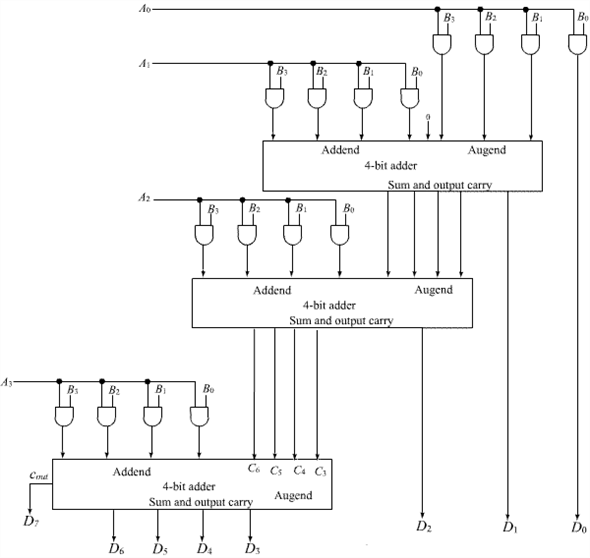
\includegraphics[scale=1]{SAT/factor/bin_mult.png}
\caption{4-bit binary multiplier}
\end{figure}

( The image has been taken from \url{http://www.chegg.com/homework-help/binary-multiplier-multiplies-two-unsigned-four-bit-numbers-u-chapter-4-problem-20p-solution-9780132774208-exc}. )

I would build separate block, "multiply by one bit" as a latch for each partial product:

\begin{lstlisting}
    def AND_Tseitin(self, v1, v2, out):
        self.add_clause([self.neg(v1), self.neg(v2), out])
        self.add_clause([v1, self.neg(out)])
        self.add_clause([v2, self.neg(out)])
    
    def AND(self,v1, v2):
        out=self.create_var()
        self.AND_Tseitin(v1, v2, out)
        return out

...

    # bit is 0 or 1.
    # i.e., if it's 0, output is 0 (all bits)
    # if it's 1, output=input
    def mult_by_bit(self, X, bit):
        return [self.AND(i, bit) for i in X]

    # bit order: [MSB..LSB]
    # build multiplier using adders and mult_by_bit blocks:
    def multiplier(self, X, Y):
        assert len(X)==len(Y)
        out=[]
        #initial:
        prev=[self.const_false]*len(X)
        # first adder can be skipped, but I left thing "as is" to make it simpler
        for Y_bit in my_utils.rvr(Y):
            s, carry = self.adder(self.mult_by_bit(X, Y_bit), prev)
            out.append(s[-1])
            prev=[carry] + s[:-1]
    
        return prev + my_utils.rvr(out)
\end{lstlisting}

AND gate is constructed here using Tseitin transformations.
This is quite popular way of encoding gates in CNF form, by adding additional variable:
\url{https://en.wikipedia.org/wiki/Tseytin_transformation}.
In fact, full-adder can be constructed without Mathematica, using logic gates, and encoded by Tseitin transformation.

\subsubsection{Glueing all together}

\lstinputlisting{SAT/factor/factor_SAT.py}
I just connect our number to output of multiplier and ask SAT solver to find inputs.
If it's UNSAT, this is prime number.
Then we factor factors recursively.

Also, we want block input factors of 1, because obviously, we do not interesting in the fact that n*1=n.
I'm using wide OR gates for this.

Output:

\begin{lstlisting}
 % python factor_SAT.py
factoring 1234567890
input_bits=31
factors of 1234567890 are 2 and 617283945
factoring 2
input_bits=1
2 is prime (unsat)
factoring 617283945
input_bits=30
factors of 617283945 are 3 and 205761315
factoring 3
input_bits=2
3 is prime (unsat)
factoring 205761315
input_bits=28
factors of 205761315 are 3 and 68587105
factoring 3
input_bits=2
3 is prime (unsat)
factoring 68587105
input_bits=27
factors of 68587105 are 5 and 13717421
factoring 5
input_bits=3
5 is prime (unsat)
factoring 13717421
input_bits=24
factors of 13717421 are 3607 and 3803
factoring 3607
input_bits=12
3607 is prime (unsat)
factoring 3803
input_bits=12
3803 is prime (unsat)
[2, 3, 3, 5, 3607, 3803]
\end{lstlisting}

So, $1234567890 = 2 \cdot 3 \cdot 3 \cdot 5 \cdot 3607 \cdot 3803$.

It works way faster than by Z3 solution, but still slow.
It can factor numbers up to maybe $\textasciitilde{}2^{40}$, while Wolfram Mathematica can factor
$\textasciitilde{}2^{80}$ easily.

% FIXME URL
The full source code: \url{https://github.com/DennisYurichev/yurichev.com/blob/master/blog/factor_SAT/factor_SAT.py}.</p>

\subsubsection{Division using multiplier}

Hard to believe, but why we couldn't define one of factors and ask SAT solver to find another factor?
Then it will divide numbers!
But, unfortunately, this is somewhat impractical, since it will work only if remainder is zero:

\lstinputlisting{SAT/factor/div.py}

% FIXME URL
The full source code: \url{https://github.com/DennisYurichev/yurichev.com/blob/master/blog/factor_SAT/div.py}.

It works very fast, but still, slower than conventional ways.

\subsubsection{Breaking \ac{RSA}}

It's not a problem to build multiplier with 4096 bit inputs and 8192 output, but it will not work in practice.
Still, you can break toy-level demonstrational RSA problems with key less than $2^{40}$ or something like that
(or larger, using Wolfram Mathematica).

\subsubsection{Further reading}

% better titles
\href{https://yurichev.com/mirrors/SAT_factor/Encoding%20Basic%20Arithmetic%20Operations%20for%20SAT-Solvers.pdf}{1},
\href{https://yurichev.com/mirrors/SAT_factor/Factoring%20integers%20with%20parallel%20SAT%20solvers.pdf}{2},
\href{https://yurichev.com/mirrors/SAT_factor/Hard%20Instance%20Generation%20for%20SAT.pdf}{3}.


\subsection{Proving bizarre XOR alternative using SAT solver}
\label{weird_XOR_SAT}

I once wrote about quite bizarre XOR alternative I've found using aha! superoptimizer: \ref{weird_XOR}.

Now let's try to prove it using SAT.

We would build an electric circuit for $x \oplus y = -2*(x \& y) + (x + y)$ like that:

% TikZ!
\begin{lstlisting}
x --- +---+
      |AND| --- +---+     
y --- +---+     |MUL| --- +---+
             -2 +---+     |ADD| --- +---+
                      x - +---+     |ADD| --> output1 --- +-------+
                                y - +---+                 |       |      +----+
                                                          |  XOR  | ---> | OR | ---> must be 0
x --- +---+                                               |       |      +----+
      |XOR| --------------------------------> output2 --- +-------+
y --- +---+
\end{lstlisting}

So it has two parts: generic XOR block and a block which must be equivalent to XOR.
Then we compare its outputs using XOR and OR.
If outputs of these parts are always equal to each other for all possible x and y, output of the whole block must be 0.

I do otherwise, I'm trying to find such an input pair, for which output will be 1:

\begin{lstlisting}
def chk1():
    input_bits=8

    s=Xu.Xu(False)

    x,y=s.alloc_BV(input_bits),s.alloc_BV(input_bits)
    step1=s.BV_AND(x,y)
    minus_2=[s.const_true]*(input_bits-1)+[s.const_false]
    product=s.multiplier(step1,minus_2)[input_bits:]
    result1=s.adder(s.adder(product, x)[0], y)[0]

    result2=s.BV_XOR(x,y)

    s.fix(s.OR(s.BV_XOR(result1, result2)), True)

    if s.solve()==False:
        print ("unsat")
        return

    print ("sat")
    print ("x=%x" % Xu.BV_to_number(s.get_BV_from_solution(x)))
    print ("y=%x" % Xu.BV_to_number(s.get_BV_from_solution(y)))
    print ("step1=%x" % Xu.BV_to_number(s.get_BV_from_solution(step1)))
    print ("product=%x" % Xu.BV_to_number(s.get_BV_from_solution(product)))
    print ("result1=%x" % Xu.BV_to_number(s.get_BV_from_solution(result1)))
    print ("result2=%x" % Xu.BV_to_number(s.get_BV_from_solution(result2)))
    print ("minus_2=%x" % Xu.BV_to_number(s.get_BV_from_solution(minus_2)))
\end{lstlisting}

% FIXME URL
The full source code: \url{https://github.com/DennisYurichev/yurichev.com/blob/master/blog/XOR_SAT/XOR_SAT.py}.

SAT solver returns "unsat", meaning, it couldn't find such a pair.
In other words, it couldn't find a counterexample.
So the circuit always outputs 0, for all possible inputs, meaning, outputs of two parts are always the same.

Modify the circuit, and the program will find such a state, and print it.

That circuit also called "miter".
According to Google translate, one of meaning of this word is:

\begin{lstlisting}
a joint made between two pieces of wood or other material at an angle of 90°, such that the line of junction bisects this angle.
\end{lstlisting}

It's also slow, because multiplier block is used: so we use small 8-bit x's and y's.

But the whole thing can be rewritten: $x \oplus y = x+y - (x \& y)<<1$.
And subtraction is addition, but with one negated operand.
So, $x \oplus y = (-(x \& y))<<1 + (x + y)$ or
$x \oplus y = (x \& y)*2 - (x + y)$.

\begin{lstlisting}
x --- +---+     +---+     +---+
      |AND| --- |NEG| --- |<<1| -+ 
y --- +---+     +---+     +---+  +- +---+
                                    |ADD| --- +---+
                                x - +---+     |ADD| --> output1 --- +-------+
                                          y - +---+                 |       |      +----+
                                                                    |  XOR  | ---> | OR | ---> must be 0
x --- +---+                                                         |       |      +----+
      |XOR| ------------------------------------------> output2 --- +-------+
y --- +---+
\end{lstlisting}

\TT{NEG} is negation block, in two's complement system.
It just inverts all bits and adds 1:

\begin{lstlisting}
    def NEG(self, x):
        # invert all bits
        tmp=self.BV_NOT(x)
        # add 1
        one=self.alloc_BV(len(tmp))
        self.fix_BV(one,n_to_BV(1, len(tmp)))
        return self.adder(tmp, one)[0]
\end{lstlisting}

Shift by one bit does nothing except rewiring.

That works way faster, and can prove correctness for 64-bit x's and y's, or for even bigger input values:

\begin{lstlisting}
def chk2():
    input_bits=64

    s=Xu.Xu(False)

    x,y=s.alloc_BV(input_bits),s.alloc_BV(input_bits)
    step1=s.BV_AND(x,y)
    step2=s.shift_left_1(s.NEG(step1))

    result1=s.adder(s.adder(step2, x)[0], y)[0]

    result2=s.BV_XOR(x,y)

    s.fix(s.OR(s.BV_XOR(result1, result2)), True)

    if s.solve()==False:
        print ("unsat")
        return

    print ("sat")
    print ("x=%x" % Xu.BV_to_number(s.get_BV_from_solution(x)))
    print ("y=%x" % Xu.BV_to_number(s.get_BV_from_solution(y)))
    print ("step1=%x" % Xu.BV_to_number(s.get_BV_from_solution(step1)))
    print ("step2=%x" % Xu.BV_to_number(s.get_BV_from_solution(step2)))
    print ("result1=%x" % Xu.BV_to_number(s.get_BV_from_solution(result1)))
    print ("result2=%x" % Xu.BV_to_number(s.get_BV_from_solution(result2)))
\end{lstlisting}

% FIXME URL
The source code: \url{https://github.com/DennisYurichev/yurichev.com/blob/master/blog/XOR_SAT/XOR_SAT.py}.


\subsection{Pocket Rubik's Cube (2*2*2) and SAT solver}
\label{PocketCubeSAT}.

I had success with my SAT-based solver, which can find an 11-turn path for a matter of 10-20 minutes on my old
Intel Xeon E3-1220 3.10GHz.

First, we will encode each color as 3-bit bit vector.
Then we can build electronic circuit, which will take initial state of cube and output final state.
It can have switches for each turn on each state.

% TODO TikZ
\begin{lstlisting}
                 +-----+    +-----+     +-----+
initial state -> | blk | -> | blk | ... | blk | -> final state
                 +-----+    +-----+     +-----+
                    ^          ^           ^
                    |          |           |
                  turn 1     turn 2    last turn
\end{lstlisting}

You set all turns and the device "calculates" final state.

Each "blk" can be constisted of 24 multiplexers (MUX), each for each facelet.
Each MUX is controlled by 5-bit command (turn number).
Depending on command, MUX takes 3-bit color from a facelet from a previous state.

Here is a table: the first column is a "destination" facelet, then a list of "source" facelets for each turn:

\begin{lstlisting}
    #      dst,  FCW  FH   FCCW UCW  UH   UCCW DCW  DH   DCCW RCW  RH   RCCW LCW  LH   LCCW BCW  BH   BCCW
    add_r("F1",["F3","F4","F2","R1","B1","L1","F1","F1","F1","F1","F1","F1","U1","B4","D1","F1","F1","F1"])
    add_r("F2",["F1","F3","F4","R2","B2","L2","F2","F2","F2","D2","B3","U2","F2","F2","F2","F2","F2","F2"])
    add_r("F3",["F4","F2","F1","F3","F3","F3","L3","B3","R3","F3","F3","F3","U3","B2","D3","F3","F3","F3"])
    add_r("F4",["F2","F1","F3","F4","F4","F4","L4","B4","R4","D4","B1","U4","F4","F4","F4","F4","F4","F4"])
    add_r("U1",["U1","U1","U1","U3","U4","U2","U1","U1","U1","U1","U1","U1","B4","D1","F1","R2","D4","L3"])
    add_r("U2",["U2","U2","U2","U1","U3","U4","U2","U2","U2","F2","D2","B3","U2","U2","U2","R4","D3","L1"])
    add_r("U3",["L4","D2","R1","U4","U2","U1","U3","U3","U3","U3","U3","U3","B2","D3","F3","U3","U3","U3"])
    add_r("U4",["L2","D1","R3","U2","U1","U3","U4","U4","U4","F4","D4","B1","U4","U4","U4","U4","U4","U4"])
    add_r("D1",["R3","U4","L2","D1","D1","D1","D3","D4","D2","D1","D1","D1","F1","U1","B4","D1","D1","D1"])
    add_r("D2",["R1","U3","L4","D2","D2","D2","D1","D3","D4","B3","U2","F2","D2","D2","D2","D2","D2","D2"])
    add_r("D3",["D3","D3","D3","D3","D3","D3","D4","D2","D1","D3","D3","D3","F3","U3","B2","L1","U2","R4"])
    add_r("D4",["D4","D4","D4","D4","D4","D4","D2","D1","D3","B1","U4","F4","D4","D4","D4","L3","U1","R2"])
    add_r("R1",["U3","L4","D2","B1","L1","F1","R1","R1","R1","R3","R4","R2","R1","R1","R1","R1","R1","R1"])
    add_r("R2",["R2","R2","R2","B2","L2","F2","R2","R2","R2","R1","R3","R4","R2","R2","R2","D4","L3","U1"])
    add_r("R3",["U4","L2","D1","R3","R3","R3","F3","L3","B3","R4","R2","R1","R3","R3","R3","R3","R3","R3"])
    add_r("R4",["R4","R4","R4","R4","R4","R4","F4","L4","B4","R2","R1","R3","R4","R4","R4","D3","L1","U2"])
    add_r("L1",["L1","L1","L1","F1","R1","B1","L1","L1","L1","L1","L1","L1","L3","L4","L2","U2","R4","D3"])
    add_r("L2",["D1","R3","U4","F2","R2","B2","L2","L2","L2","L2","L2","L2","L1","L3","L4","L2","L2","L2"])
    add_r("L3",["L3","L3","L3","L3","L3","L3","B3","R3","F3","L3","L3","L3","L4","L2","L1","U1","R2","D4"])
    add_r("L4",["D2","R1","U3","L4","L4","L4","B4","R4","F4","L4","L4","L4","L2","L1","L3","L4","L4","L4"])
    add_r("B1",["B1","B1","B1","L1","F1","R1","B1","B1","B1","U4","F4","D4","B1","B1","B1","B3","B4","B2"])
    add_r("B2",["B2","B2","B2","L2","F2","R2","B2","B2","B2","B2","B2","B2","D3","F3","U3","B1","B3","B4"])
    add_r("B3",["B3","B3","B3","B3","B3","B3","R3","F3","L3","U2","F2","D2","B3","B3","B3","B4","B2","B1"])
    add_r("B4",["B4","B4","B4","B4","B4","B4","R4","F4","L4","B4","B4","B4","D1","F1","U1","B2","B1","B3"])
\end{lstlisting}

Each MUX has 32 inputs, each has width of 3 bits: colors from "source" facelets.
It has 3-bit output (color for "destination" facelet).
It has 5-bit selector, for 18 turns. Other selector values (32-18=14 values) are not used at all.

The whole problem is to build a circuit and then ask SAT solver to set "switches" to such a state,
when input and output are determined (by us).

Now the problem is to represent MUX in CNF terms.

From \ac{EE} courses we can remember about a simple if-then-else (ITE) gate, it takes 3 inputs
("selector", "true" and "false") and it has 1 output.
Depending on "selector" input it "connects" output with "true" or "false" input.
Using tree of ITE gates we first can build 32-to-1 MUX, then wide 32*3-to-3 MUX.

% FIXME URL
I once have written small utility to search for shortest possible CNF formula for a specific function,
in a bruteforce manner (\url{https://github.com/DennisYurichev/yurichev.com/blob/master/blog/rubik/XOR_CNF_bf.c}).
It was inspired by "aha! hacker assistant" by Henry Warren.
So here is a function:

\begin{lstlisting}
bool func(bool v[VARIABLES])
{

	// ITE:

	bool tmp;
	if (v[0]==0)
		tmp=v[1];
	else
		tmp=v[2];

	return tmp==v[3];
}
\end{lstlisting}

A shortest CNF for it:

\begin{lstlisting}
try_all_CNFs_of_len(1)
try_all_CNFs_of_len(2)
try_all_CNFs_of_len(3)
try_all_CNFs_of_len(4)
found a CNF:
p cnf 4 4
-1 3 -4 0
1 2 -4 0
-1 -3 4 0
1 -2 4 0
\end{lstlisting}

1st variable is "select", 2nd is "false", 3rd is "true", 4th is "output".
"output" is an additional variable, added just like in Tseitin transformations.

Hence, CNF formula is:

\begin{lstlisting}
(!select OR true OR !output) AND (select OR false OR !output) AND (!select OR !true OR output) AND (select OR !false OR output)
\end{lstlisting}

It assures that the "output" will always be equal to one of inputs depending on "select".

Now we can build a tree of ITE gates:

\begin{lstlisting}
def create_ITE(s,f,t):
    x=create_var()

    clauses.append([neg(s),t,neg(x)])
    clauses.append([s,f,neg(x)])
    clauses.append([neg(s),neg(t),x])
    clauses.append([s,neg(f),x])

    return x

# ins=16 bits
# sel=4 bits
def create_MUX(ins, sel):
    t0=create_ITE(sel[0],ins[0],ins[1])
    t1=create_ITE(sel[0],ins[2],ins[3])
    t2=create_ITE(sel[0],ins[4],ins[5])
    t3=create_ITE(sel[0],ins[6],ins[7])
    t4=create_ITE(sel[0],ins[8],ins[9])
    t5=create_ITE(sel[0],ins[10],ins[11])
    t6=create_ITE(sel[0],ins[12],ins[13])
    t7=create_ITE(sel[0],ins[14],ins[15])

    y0=create_ITE(sel[1],t0,t1)
    y1=create_ITE(sel[1],t2,t3)
    y2=create_ITE(sel[1],t4,t5)
    y3=create_ITE(sel[1],t6,t7)

    z0=create_ITE(sel[2],y0,y1)
    z1=create_ITE(sel[2],y2,y3)

    return create_ITE(sel[3], z0, z1)
\end{lstlisting}

This is my old MUX I wrote for 16 inputs and 4-bit selector, but you've got the idea: this is 4-tier tree.
It has 15 ITE gates or 15*4=60 clauses.

Now the question, is it possible to make it smaller?
I've tried to use Mathematica.
First I've built truth table for 4-bit selector:

\begin{lstlisting}
...
1 1 1 1     1 1 1 1 1 1 0 1 0 1 0 1 1 0 1 1    0    0
1 1 1 1     1 1 1 1 1 1 0 1 0 1 0 1 1 0 1 1    1    1
1 1 1 1     1 1 1 1 1 1 0 1 0 1 0 1 1 1 0 0    0    0
1 1 1 1     1 1 1 1 1 1 0 1 0 1 0 1 1 1 0 0    1    1
1 1 1 1     1 1 1 1 1 1 0 1 0 1 0 1 1 1 0 1    0    0
1 1 1 1     1 1 1 1 1 1 0 1 0 1 0 1 1 1 0 1    1    1
1 1 1 1     1 1 1 1 1 1 0 1 0 1 0 1 1 1 1 0    0    0
1 1 1 1     1 1 1 1 1 1 0 1 0 1 0 1 1 1 1 0    1    1
1 1 1 1     1 1 1 1 1 1 0 1 0 1 0 1 1 1 1 1    0    0
1 1 1 1     1 1 1 1 1 1 0 1 0 1 0 1 1 1 1 1    1    1
1 1 1 1     1 1 1 1 1 1 0 1 0 1 1 0 0 0 0 0    0    0
1 1 1 1     1 1 1 1 1 1 0 1 0 1 1 0 0 0 0 0    1    1
1 1 1 1     1 1 1 1 1 1 0 1 0 1 1 0 0 0 0 1    0    0
1 1 1 1     1 1 1 1 1 1 0 1 0 1 1 0 0 0 0 1    1    1
1 1 1 1     1 1 1 1 1 1 0 1 0 1 1 0 0 0 1 0    0    0
1 1 1 1     1 1 1 1 1 1 0 1 0 1 1 0 0 0 1 0    1    1
1 1 1 1     1 1 1 1 1 1 0 1 0 1 1 0 0 0 1 1    0    0
...
\end{lstlisting}

First 4 bits is selector, then 16 bits of input.
Then the possible output and the bit, indicating, if the output bit equals to one of the inputs.

Then I load this table to Mathematica and make CNF expression out of truth table:

\begin{lstlisting}
arr=Import["/home/dennis/P/Rubik/TT","Table"]
{{0,0,0,0,0,0,0,0,0,0,0,0,0,0,0,0,0,0,0,0,0,1},{0,0,0,0,0,0,0,0,0,0,0,0,0,0,0,0,0,0,0,0,1,0},{0,0,0,0,0,0,0,0,0,0,0,0,0,0,0,0,0,0,0,1,0,0},
{0,0,0,0,0,0,0,0,0,0,0,0,0,0,0,0,0,0,0,1,1,1},{0,0,0,0,0,0,0,0,0,0,0,0,0,0,0,0,0,0,1,0,0,1},{0,0,0,0,0,0,0,0,0,0,0,0,0,0,0,0,0,0,1,0,1,0},
{0,0,0,0,0,0,0,0,0,0,0,0,0,0,0,0,0,0,1,1,0,0},{0,0,0,0,0,0,0,0,0,0,0,0,0,0,0,0,0,0,1,1,1,1},{0,0,0,0,0,0,0,0,0,0,0,0,0,0,0,0,0,1,0,0,0,1}, ⋯2097135⋯ ,
{1,1,1,1,1,1,1,1,1,1,1,1,1,1,1,1,1,1,0,0,0,0},{1,1,1,1,1,1,1,1,1,1,1,1,1,1,1,1,1,1,0,0,1,1},{1,1,1,1,1,1,1,1,1,1,1,1,1,1,1,1,1,1,0,1,0,0},
{1,1,1,1,1,1,1,1,1,1,1,1,1,1,1,1,1,1,0,1,1,1},{1,1,1,1,1,1,1,1,1,1,1,1,1,1,1,1,1,1,1,0,0,0},{1,1,1,1,1,1,1,1,1,1,1,1,1,1,1,1,1,1,1,0,1,1},
{1,1,1,1,1,1,1,1,1,1,1,1,1,1,1,1,1,1,1,1,0,0},{1,1,1,1,1,1,1,1,1,1,1,1,1,1,1,1,1,1,1,1,1,1}}


TT=(Most[#]->Last[#])&/@arr
{{0,0,0,0,0,0,0,0,0,0,0,0,0,0,0,0,0,0,0,0,0}->1,{0,0,0,0,0,0,0,0,0,0,0,0,0,0,0,0,0,0,0,0,1}->0,{0,0,0,0,0,0,0,0,0,0,0,0,0,0,0,0,0,0,0,1,0}->0,
{0,0,0,0,0,0,0,0,0,0,0,0,0,0,0,0,0,0,0,1,1}->1,{0,0,0,0,0,0,0,0,0,0,0,0,0,0,0,0,0,0,1,0,0}->1,{0,0,0,0,0,0,0,0,0,0,0,0,0,0,0,0,0,0,1,0,1}->0,
{0,0,0,0,0,0,0,0,0,0,0,0,0,0,0,0,0,0,1,1,0}->0,{0,0,0,0,0,0,0,0,0,0,0,0,0,0,0,0,0,0,1,1,1}->1,{0,0,0,0,0,0,0,0,0,0,0,0,0,0,0,0,0,1,0,0,0}->1, ⋯2097135⋯ ,
{1,1,1,1,1,1,1,1,1,1,1,1,1,1,1,1,1,1,0,0,0}->0,{1,1,1,1,1,1,1,1,1,1,1,1,1,1,1,1,1,1,0,0,1}->1,{1,1,1,1,1,1,1,1,1,1,1,1,1,1,1,1,1,1,0,1,0}->0,
{1,1,1,1,1,1,1,1,1,1,1,1,1,1,1,1,1,1,0,1,1}->1,{1,1,1,1,1,1,1,1,1,1,1,1,1,1,1,1,1,1,1,0,0}->0,{1,1,1,1,1,1,1,1,1,1,1,1,1,1,1,1,1,1,1,0,1}->1,
{1,1,1,1,1,1,1,1,1,1,1,1,1,1,1,1,1,1,1,1,0}->0,{1,1,1,1,1,1,1,1,1,1,1,1,1,1,1,1,1,1,1,1,1}->1}


BooleanConvert[BooleanFunction[TT,{s3,s2,s1,s0, i15,i14,i13,i12,i11,i10,i9,i8,i7,i6,i5,i4,i3, i2, i1, i0,x}],"CNF"]
(!i0||s0||s1||s2||s3||x)&&(i0||s0||s1||s2||s3||!x)&&(!i1||!s0||s1||s2||s3||x)&&(i1||!s0||s1||s2||s3||!x)&&(!i10||s0||!s1||s2||!s3||x)&&
(i10||s0||!s1||s2||!s3||!x)&&(!i11||!s0||!s1||s2||!s3||x)&&(i11||!s0||!s1||s2||!s3||!x)&&(!i12||s0||s1||!s2||!s3||x)&&(i12||s0||s1||!s2||!s3||!x)&&
(!i13||!s0||s1||!s2||!s3||x)&&(i13||!s0||s1||!s2||!s3||!x)&&(!i14||s0||!s1||!s2||!s3||x)&&(i14||s0||!s1||!s2||!s3||!x)&&
(!i15||!s0||!s1||!s2||!s3||x)&&(i15||!s0||!s1||!s2||!s3||!x)&&(!i2||s0||!s1||s2||s3||x)&&(i2||s0||!s1||s2||s3||!x)&&(!i3||!s0||!s1||s2||s3||x)&&
(i3||!s0||!s1||s2||s3||!x)&&(!i4||s0||s1||!s2||s3||x)&&(i4||s0||s1||!s2||s3||!x)&&(!i5||!s0||s1||!s2||s3||x)&&(i5||!s0||s1||!s2||s3||!x)&&
(!i6||s0||!s1||!s2||s3||x)&&(i6||s0||!s1||!s2||s3||!x)&&(!i7||!s0||!s1||!s2||s3||x)&&(i7||!s0||!s1||!s2||s3||!x)&&(!i8||s0||s1||s2||!s3||x)&&
(i8||s0||s1||s2||!s3||!x)&&(!i9||!s0||s1||s2||!s3||x)&&(i9||!s0||s1||s2||!s3||!x)
\end{lstlisting}

Look closer to CNF expression:

\begin{lstlisting}
(!i0|   |s0||s1||s2|| s3|| x)&&
( i0||  s0|| s1||s2|| s3||!x)&&
(!i1||! s0|| s1||s2|| s3|| x)&&
( i1||! s0|| s1||s2|| s3||!x)&&
(!i10|| s0||!s1||s2||!s3|| x)&&
( i10|| s0||!s1||s2||!s3||!x)&&
(!i11||!s0||!s1||s2||!s3|| x)&&
( i11||!s0||!s1||s2||!s3||!x)&&

...

(!i8|| s0||s1||s2||!s3|| x)&&
( i8|| s0||s1||s2||!s3||!x)&&
(!i9||!s0||s1||s2||!s3|| x)&&
( i9||!s0||s1||s2||!s3||!x)
\end{lstlisting}

It has simple structure and there are 32 clauses, against 60 in my previous attempt.
Will it work faster?
No, as my experience shows, it doesn't speed up anything.
Anyway, I used the latter idea to make MUX.

The following function makes pack of MUXes for each state, based on what I've got from Mathematica:

\begin{lstlisting}
    def create_MUX(self, ins, sels):
        assert 2**len(sels)==len(ins)
        x=self.create_var()
        for sel in range(len(ins)): # 32 for 5-bit selector
            tmp=[self.neg_if((sel>>i)&1==1, sels[i]) for i in range(len(sels))] # 5 for 5-bit selector
    
            self.add_clause([self.neg(ins[sel])] + tmp + [x])
            self.add_clause([ins[sel]] + tmp + [self.neg(x)])
        return x
    
    def create_wide_MUX (self, ins, sels):
        out=[]
        for i in range(len(ins[0])):
            inputs=[x[i] for x in ins]
            out.append(self.create_MUX(inputs, sels))
        return out
\end{lstlisting}

% FIXME URL to Xu.py

Now the function that glues all together:

\begin{lstlisting}
# src=list of 18 facelets
def add_r(dst, src):
    global facelets, selectors, s
    t=s.create_var()
    s.fix(t,True)
    for state in range(STATES-1):
        src_vectors=[]
        for tmp in src:
            src_vectors.append(facelets[state][tmp])

        # padding: there are 18 used MUX inputs, so add 32-18=14 for padding
        for i in range(32-18): 
            src_vectors.append([t,t,t])

        dst_vector=s.create_wide_MUX (src_vectors, selectors[state])
        s.fix_BV_EQ(dst_vector,facelets[state+1][dst])

...

    #      dst,  FCW  FH   FCCW UCW  UH   UCCW DCW  DH   DCCW RCW  RH   RCCW LCW  LH   LCCW BCW  BH   BCCW
    add_r("F1",["F3","F4","F2","R1","B1","L1","F1","F1","F1","F1","F1","F1","U1","B4","D1","F1","F1","F1"])
    add_r("F2",["F1","F3","F4","R2","B2","L2","F2","F2","F2","D2","B3","U2","F2","F2","F2","F2","F2","F2"])
    add_r("F3",["F4","F2","F1","F3","F3","F3","L3","B3","R3","F3","F3","F3","U3","B2","D3","F3","F3","F3"])
    add_r("F4",["F2","F1","F3","F4","F4","F4","L4","B4","R4","D4","B1","U4","F4","F4","F4","F4","F4","F4"])
    add_r("U1",["U1","U1","U1","U3","U4","U2","U1","U1","U1","U1","U1","U1","B4","D1","F1","R2","D4","L3"])
...
\end{lstlisting}

% FIXME URL
Now the full source code: \url{https://github.com/DennisYurichev/yurichev.com/blob/master/blog/rubik/SAT.py}.
I tried to make it as concise as possible.
It requires minisat to be installed.

And it works up to 11 turns, starting at 11, then decreasing number of turns.
Here is an output for a state which can be solved with 4 turns:

\begin{lstlisting}
set_state(0, {"F":"RYOG", "U":"YRGO", "D":"WRBO", "R":"GYWB", "L":"BYWG", "B":"BOWR"})
\end{lstlisting}

\lstinputlisting{SAT/rubik2/post_RDUR.txt}

Even on my relic Intel Atom 1.5GHz netbook it takes just 20s.

You can find redundant turns in 11-turn solution, like double UH turns.
Of course, two UH turns returns the cube to the previous state.
So these "annihilating turns" are added if the final solution can be shorter.
Why the solver added it? There is no "no operation" turn. And the solver is forced to fit into 11 turns.
Hence, it do what it can to produce correct solution.

Now a hard example:

\begin{lstlisting}
set_state(0, {"F":"RORW", "U":"BRBB", "D":"GOOR", "R":"WYGY", "L":"OWYW", "B":"BYGG"})
\end{lstlisting}

\begin{lstlisting}
TURNS= 11
sat!
UCW
BCW
LCCW
BH
DCW
RH
DCCW
FCW
UH
LCW
RCW

TURNS= 10
sat!
RH
BCCW
LCCW
RH
BCCW
LH
BCW
DH
BCW
LCCW

...
\end{lstlisting}

( ~5m on my old Intel Xeon E3-1220 3.10GHz. )

I couldn't find a pure "11-turn state" which is "unsat" for 10-turn, it seems, these are rare.
According to \href{https://en.wikipedia.org/wiki/Pocket_Cube}{wikipedia}, there are just 0.072\% of these states.
Like "20-turn states" for 3*3*3 cube, which are also rare.

\subsubsection{Several solutions}

According to picosat (--all option to get all possible solutions), the 4-turn example we just saw has 2 solutions.
Indeed, two consequent turns UCW and DCW can be interchanged, they do not conflict with each other.

\subsubsection{Other (failed) ideas}

Pocket cube (2*2*2) has no central facelets, so to solve it, you don't need to stick each color to each face.
Rather, you can define a constraint so that a colors on each face must be equal to each other.
Somehow, this slows down drastically my both Z3 and SAT-based solvers.

Also, to prevent "annihilating" turns, we can set a constraint so that each state cannot be equal to any of previous
states, i.e., states cannot repeat.
This also slows down my both solvers.

\subsubsection{3*3*3 cube}

3*3*3 cube requires much more turns (20), so I couldn't solve it with my methods.
I have success to solve maybe 10 or 11 turns.
But some people do all 20 turns: \href{https://arxiv.org/pdf/1105.1436.pdf}{Jingchao Chen}.

However, you can use 3*3*3 cube to play, because it can act as 2*2*2 cube: just use corners and ignore
edge and center cubes.
Here is mine I used, you can see that corners are correctly solved:

\begin{figure}[H]
\centering
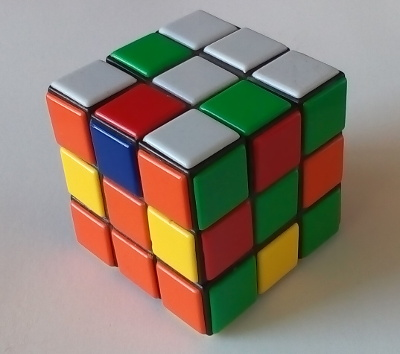
\includegraphics[scale=0.75]{SAT/rubik2/3solved.jpg}
\caption{Rubik's cube as pocket cube}
\end{figure}

\subsubsection{Some discussion}

\url{https://news.ycombinator.com/item?id=15214439},\\
\url{https://www.reddit.com/r/compsci/comments/6zb34i/solving_pocket_rubiks_cube_222_using_z3_and_sat/},\\
\url{https://www.reddit.com/r/Cubers/comments/6ze3ua/theory_dennis_yurichev_solving_pocket_rubiks_cube/}.


\subsection{List of SAT-solvers}

% TODO authors, URLs

\begin{itemize}

\item MiniSat\footnote{http://minisat.se/}, serving as a base for others

\item PicoSat, PrecoSat, Lingeling. Created by Armin Biere. Plingeling supports multithreading.

\item CryptoMiniSat. Created by Mate Soos for cryptographical problems exploration.
Supports XOR clauses, multithreading.
Has Python API.

\end{itemize}



